% CSL7620 course project report in CVPR format (official author kit: https://github.com/cvpr-org/author-kit)
% Build: pdflatex main; bibtex main; pdflatex main; pdflatex main
\documentclass[10pt,twocolumn,letterpaper]{article}

\usepackage[pagenumbers]{cvpr}   % camera-ready layout with page numbers (course report, not a CVPR submission)
%% This file contains a number of tweaks that are typically applied to the main document.
%% They are not enabled by default, but can be enabled by uncommenting the relevant lines.


%%
%% Official support for 2-column teaser figure
%%
\usepackage{cuted} %< for strip environment

%%
%% For auto-referencing of figures (see fig/teaser.tex and \label{} therein) 
%%
\usepackage{currfile} %< for \currfilebase macro

%%
%% caption and (global) spacing overrides
%%
\usepackage{caption} %< for "\captionof" commands (teaser)
% \setlength{\abovecaptionskip}{.5em} % space above caption
% \setlength{\belowcaptionskip}{1em} % space below caption

%%
%% Inline annotations; for predefined colors, refer to "dvipsnames" in the xcolor package:
%% https://tinyurl.com/overleaf-colors
%%
\newcommand{\red}[1]{{\color{red}#1}}
\newcommand{\todo}[1]{{\color{red}#1}}
\newcommand{\TODO}[1]{\textbf{\color{red}[TODO: #1]}}
%%
%% Disable for camera ready / submission by uncommenting these lines:
%%
% \renewcommand{\TODO}[1]{}
% \renewcommand{\todo}[1]{#1}

%%
%% Work harder in optimizing text layout. Typically shrinks text by 1/6 of page, enable
%% it at the very end of the writing process, when you are just above the page limit.
%%
% \usepackage{microtype}

%%
%% Fine-tune paragraph spacing.
%%
% \renewcommand{\paragraph}[1]{\vspace{.5em}\noindent\textbf{#1.}}

%%
%% Globally adjusts space between figure and caption.
%%
% \setlength{\abovecaptionskip}{.5em}

%%
%% Allows "the use of \paper to refer to the project name"
%% with automatic management of space at the end of the word.
%%
% \usepackage{xspace}
% \newcommand{\paper}{ProjectName\xspace}

%%
%% Commonly used math definitions.
%%
% \DeclareMathOperator*{\argmin}{arg\,min}
% \DeclareMathOperator*{\argmax}{arg\,max}

%%
%% Tighten underline.
%%
% \usepackage{soul}
% \setuldepth{foobar}

%%
%% Fix misplaced line numbers with lineno v5.7/v5.8 (Feb 2026, e.g. early TeX Live 2026 installs).
%% These versions write the column tag outside the column box, so line numbers end up on the
%% wrong side of the column. This backports the fix from lineno v5.9 and does nothing for other
%% lineno versions or in camera-ready mode. Updating TeX Live (tlmgr update --all) also fixes it.
%%
\makeatletter
\@ifpackageloaded{lineno}{\ifdefined\IfFormatAtLeastTF\IfFormatAtLeastTF{2025-06-01}{%
  \@ifpackagelater{lineno}{2026/03/08}{}{\@ifpackagelater{lineno}{2026/02/16}{%
    \RemoveFromHook{build/column/before}[lineno]%
    \AddToHook{build/column/after}{%
      \setbox\@outputbox\vbox to\ht\@outputbox{%
        \boxmaxdepth\@maxdepth
        \protected@write\@auxout{}{%
          \string\def\string\@LN@column{\if@firstcolumn1\else2\fi}}%
        \unvbox\@outputbox}}%
  }{}}}{}\fi}{}
\makeatother

\usepackage{booktabs}
\usepackage{multirow}
\usepackage{amsmath}
\definecolor{cvprblue}{rgb}{0.21,0.49,0.74}
\usepackage[pagebackref,breaklinks,colorlinks,allcolors=cvprblue]{hyperref}

\def\confName{CSL7620}
\def\confYear{2026}
\def\repoURL{https://github.com/RahulBhikundia/enose-drift-benchmark}

\title{Does Flatness Help Gas Sensors Survive Drift?\\
{\large A Leakage-Free Benchmark of Sharpness-Aware, Domain-Generalization and\\Test-Time Adaptation Methods under Real Electronic-Nose Drift}}

\author{Rahul Bhikundia\\
{M26CSA006}\\
IIT Jodhpur
\and
Gourav\\
{M26CSE018}\\
IIT Jodhpur
\and
Jharendra Jogi\\
{M26MAC005}\\
IIT Jodhpur
}

\begin{document}
\maketitle

% ====================================================================== abstract
\begin{abstract}
Metal-oxide gas sensors drift: they age, and two copies of the same device never respond identically, so a
classifier trained on yesterday's data degrades on tomorrow's. Flat minima, found by sharpness-aware minimization
(SAM) and its cheap variant Momentum-SAM (MSAM), are often claimed to generalize better under distribution shift. We
test that claim on real drift. After auditing three public datasets covering three drift types---sensor ageing (UCI
Gas Sensor Array Drift), session-to-session shift (SmellNet) and device-to-device shift (UCI Twin Gas Sensor
Arrays)---we compare about 20 methods under one frozen protocol: equal tuning budget, selection on validation only,
a single test pass with 5--10 seeds, and statistics over held-out domains. No sharpness-aware or
domain-generalization method reliably beats AdamW; MSAM is as cheap as SGD but unstable, and a drift-aware MSAM
variant we propose does not beat a random-direction control. Validation-based selection is unreliable under drift.
What does help depends on the drift type: an oracle per-sensor calibration diagnosis shows that device shift is
calibration-type, and label-free test-time adaptation there matches labelled recalibration (Twin
$0.910\!\rightarrow\!0.982$ macro-F1) and recovers most of it for session shift (SmellNet
$0.851\!\rightarrow\!0.918$). Ageing is different: only a few labelled samples from the new period help (UCI
$0.763\!\rightarrow\!0.929$; best label-free $0.784$). The remedy should be matched to the drift type.
\end{abstract}

% ====================================================================== 1 intro
\section{Introduction}
\label{sec:intro}
An electronic nose (e-nose) is an array of chemical sensors whose joint response is a fingerprint of a gas. Over
weeks and months the sensors' baselines and sensitivities change (ageing, poisoning, humidity and temperature
effects), and manufacturing tolerances make every unit respond slightly differently. A model trained on one period
or one device therefore faces a shifted input distribution in deployment, and recalibrating sensors with reference
gases is expensive.

Sharpness-aware minimization (SAM)~\cite{foret2021sam} seeks weights whose loss stays low in a whole neighbourhood
(a ``flat'' minimum), and flatness is frequently linked to robustness under distribution
shift~\cite{wang2023sagm,zhang2024disam}. SAM needs a second forward/backward pass per step; Momentum-SAM
(MSAM)~\cite{becker2024msam} perturbs along the momentum direction and is almost free. If flatness bought drift
robustness, MSAM would be a free fix. The UCI benchmark, however, is temporally confounded~\cite{dennler2022drift},
so any such claim needs a careful protocol.

We test the claim on all three drift types available in public e-nose data, against the method families a
practitioner would try. Our contributions are:
\begin{itemize}
\item A leakage-audited benchmark of the SAM family (SAM, MSAM, SAGM, DISAM), domain-generalization (DG) methods and
classical baselines on three real drift types under one frozen, validation-only protocol (\cref{sec:data,sec:protocol}).
\item SA-MSAM, a drift-aware MSAM variant, tested against a random-direction control with a pre-registered go/no-go;
it is a negative result (\cref{sec:samsam}).
\item Evidence that validation-based selection is unreliable under drift and that sharpness barely predicts
robustness (\cref{sec:selection}).
\item An oracle-calibration shift diagnosis and a controlled comparison showing that the same label-free test-time
adaptation (TTA) works for device and session shift but not for ageing (\cref{sec:diag,sec:tta}).
\end{itemize}

% ====================================================================== 2 related
\section{Related Work}
\label{sec:related}
\paragraph{Sharpness-aware optimization.} SAM~\cite{foret2021sam} minimizes the worst-case loss in an $\ell_2$ ball
of radius $\rho$ around the weights. MSAM~\cite{becker2024msam} replaces the gradient-ascent perturbation by the
normalized negative momentum, removing the extra pass. SAGM~\cite{wang2023sagm} aligns the gradients of the
empirical and perturbed losses for DG; DISAM~\cite{zhang2024disam} balances per-domain losses inside the
perturbation. These were evaluated mostly on image DG benchmarks. SAM has been used inside a domain-adversarial
network for e-nose drift\footnote{Sensors 24(4):1319, 2024.}, but we found no head-to-head comparison with DG and
adaptation methods across several real drift types.

\paragraph{Domain generalization and model selection.} CORAL~\cite{sun2016coral} aligns second-order feature
statistics; GroupDRO~\cite{sagawa2020groupdro} up-weights the worst domain; SWA~\cite{izmailov2018swa} averages
weights. DomainBed~\cite{gulrajani2021domainbed} showed that, under fair selection, empirical risk minimization is
hard to beat on images. We confirm this on sensor data.

\paragraph{E-nose drift compensation.} Vergara \etal~\cite{vergara2012drift} introduced the UCI drift dataset;
domain-adaptation methods followed, \eg~\cite{zhang2015daelm}. Dennler \etal~\cite{dennler2022drift} showed that
UCI is confounded by acquisition time. Fonollosa \etal~\cite{fonollosa2016twin} introduced the Twin dataset with
supervised direct standardization. SmellNet~\cite{feng2025smellnet} is a recent large real-world dataset. Fu
\etal~\cite{fu2026protocol} report that compensation rankings depend on chronology and target-data availability, in
line with our selection results.

\paragraph{Test-time adaptation.} Tent~\cite{wang2021tent} minimizes prediction entropy at test time;
SHOT~\cite{liang2020shot} adapts the feature extractor with an information-maximization (IM) objective and a frozen
classifier. Online TTA was recently proposed for e-nose drift~\cite{liang2024otta,liang2025otta}. We do not propose
a TTA method; we ask on which drift types standard ones work, and why.

% ====================================================================== 3 data
\section{Datasets and Leakage Audit}
\label{sec:data}
\begin{table}[t]
\centering\footnotesize\setlength{\tabcolsep}{3pt}
\begin{tabular}{@{}llll@{}}
\toprule
 & UCI Drift~\cite{vergara2012drift} & SmellNet~\cite{feng2025smellnet} & Twin~\cite{fonollosa2016twin} \\
\midrule
Drift & ageing, 36 mo. & session (day) & device (unit) \\
Domains & 10 batches & 6 sessions & 5 units \\
Input & 128 features & $100\times6$ window & 64 features \\
Task & 6 gases & 50 substances & 4 gases / conc. \\
Metric & macro-F1 & macro-F1 & macro-F1 / $R^2$ \\
Test splits & 1--5$\to$6--10, & leave one & leave one \\
 & + 8 rolling & session out & unit out \\
Model & MLP & 1-D CNN & MLP \\
\bottomrule
\end{tabular}
\caption{Datasets. Tuning splits: UCI train 1--3/val 4--5; SmellNet train 1--4/val 5; Twin train units 1--3/val 4.}
\label{tab:data}
\end{table}
\Cref{tab:data} summarizes the data. We use all of SmellNet-Base (50 substances $\times$ 6 sessions; its mixture and
GC-MS subsets address other tasks) and extract 8 features per sensor from the raw Twin recordings, after resampling
the 82 of 640 irregularly sampled files to a uniform grid. Before any method was run we audited each dataset.

\paragraph{Random splits leak heavily.} UCI reaches 99.4\% accuracy with a random 80/20 split but 47--77\% when
training on the past and testing on the future. SmellNet reaches 99.9\% on random windows but $\approx$82\% on an
unseen session, because overlapping windows of one recording fall on both sides. Twin concentration reaches $R^2$
0.81--0.94 on random splits and is negative on some unseen units. \emph{All results use domain-held-out splits},
with scalers fitted on training domains only.

\paragraph{Drift is strong and not monotonic.} A linear classifier separates UCI batch~1 from every later batch at
97--100\%, yet batch~10 moves back towards batch~1. SmellNet sessions and Twin units are identifiable at
$\geq$99.5\%. Toluene is absent from UCI batches 3--5, so macro-F1 is computed over the classes present. The
pre-exposure baseline needed for the test of~\cite{dennler2022drift} is not in the 128-feature release, so we do
not claim to have run it.

% ====================================================================== 4 methods
\section{Methods}
\label{sec:methods}
We compare SGD with momentum, AdamW~\cite{loshchilov2019adamw} (reference) and a random forest; SAM, MSAM, SAGM and
DISAM; CORAL, GroupDRO and mixed-domain batches; recency weighting and time as an input; per-domain normalization,
class-conditional PCA drift removal (CC-PCA) and gain/offset drift augmentation; and SWA (early-stopped and
full-length). Methods that use unlabelled target data are marked transductive.

\paragraph{SA-MSAM.} MSAM perturbs the weights by $\epsilon = -\rho\, m/\lVert m\rVert$ with momentum $m$.
SA-MSAM replaces $m$ by an estimate of the drift direction in gradient space: the difference between the mean
gradients of the newest and oldest training domains (\emph{extrapolated}) or the direction of maximal disagreement
between domains. A random unit direction of the same norm is the control.

\paragraph{Few-shot recalibration.} The frozen AdamW model is recalibrated with $k$ labelled target samples by a
per-feature affine map, by fine-tuning the last layer, or by fine-tuning all layers.

\paragraph{Label-free test-time adaptation.} Given the frozen source model and the unlabelled samples of one target
domain: \emph{standardize} re-standardizes each input feature with target statistics; \emph{feature alignment}
matches the mean and standard deviation of the penultimate features to the source; \emph{entropy input-affine}
learns a per-feature input gain and offset by minimizing the IM loss
\begin{equation}
\mathcal{L}_{\text{IM}} = \tfrac{1}{n}\textstyle\sum_i H\big(p(y\,|\,x_i)\big) - H\big(\tfrac{1}{n}\sum_i p(y\,|\,x_i)\big);
\end{equation}
\emph{SHOT-IM}~\cite{liang2020shot} updates the feature extractor with the same loss and a frozen classifier. TTA
learning rates and steps were chosen on the validation split. The reference is few-shot fine-tuning of all layers
($k$ = 5 per class on UCI, the first 4 windows per recording on SmellNet, 2 recordings per gas on Twin).

\paragraph{Shift diagnosis.} We correct the test inputs with per-feature maps of increasing power, up to an
\emph{oracle} gain and offset fitted with the test labels. It is a diagnostic upper bound for calibration-type
correction, never used for selection: if even the oracle calibration does not help, the shift is not a per-sensor
calibration error.

% ====================================================================== 5 protocol
\section{Experimental Protocol}
\label{sec:protocol}
Every method gets the same budget of 12 hyperparameter configurations $\times$ 3 seeds on the tuning split; the
configuration with the best mean validation score is selected and the number of epochs is the median
best-validation epoch. Settings are frozen before any test run, every method is reported including collapses, and
test runs use 5 seeds (UCI, SmellNet) or 10 seeds (Twin) on every held-out split. All SAM-family methods share an
SGD-momentum base; our MSAM matches the official code to $10^{-10}$. No BatchNorm is used, as it interacts with
perturbed passes. The unit of analysis is the held-out split: against AdamW we report the mean difference, a 95\%
bootstrap CI over splits, the number of splits won, Wilcoxon signed-rank tests with Holm correction and Friedman
tests. Twin-concentration runs that diverged are scored $R^2=0$. Every run writes a JSON record; decisions are
dated in a log. In total we trained $\approx$7{,}200 models on one laptop GPU.

% ====================================================================== 6 results
\section{Results}
\label{sec:results}

\begin{figure*}[t]
\centering
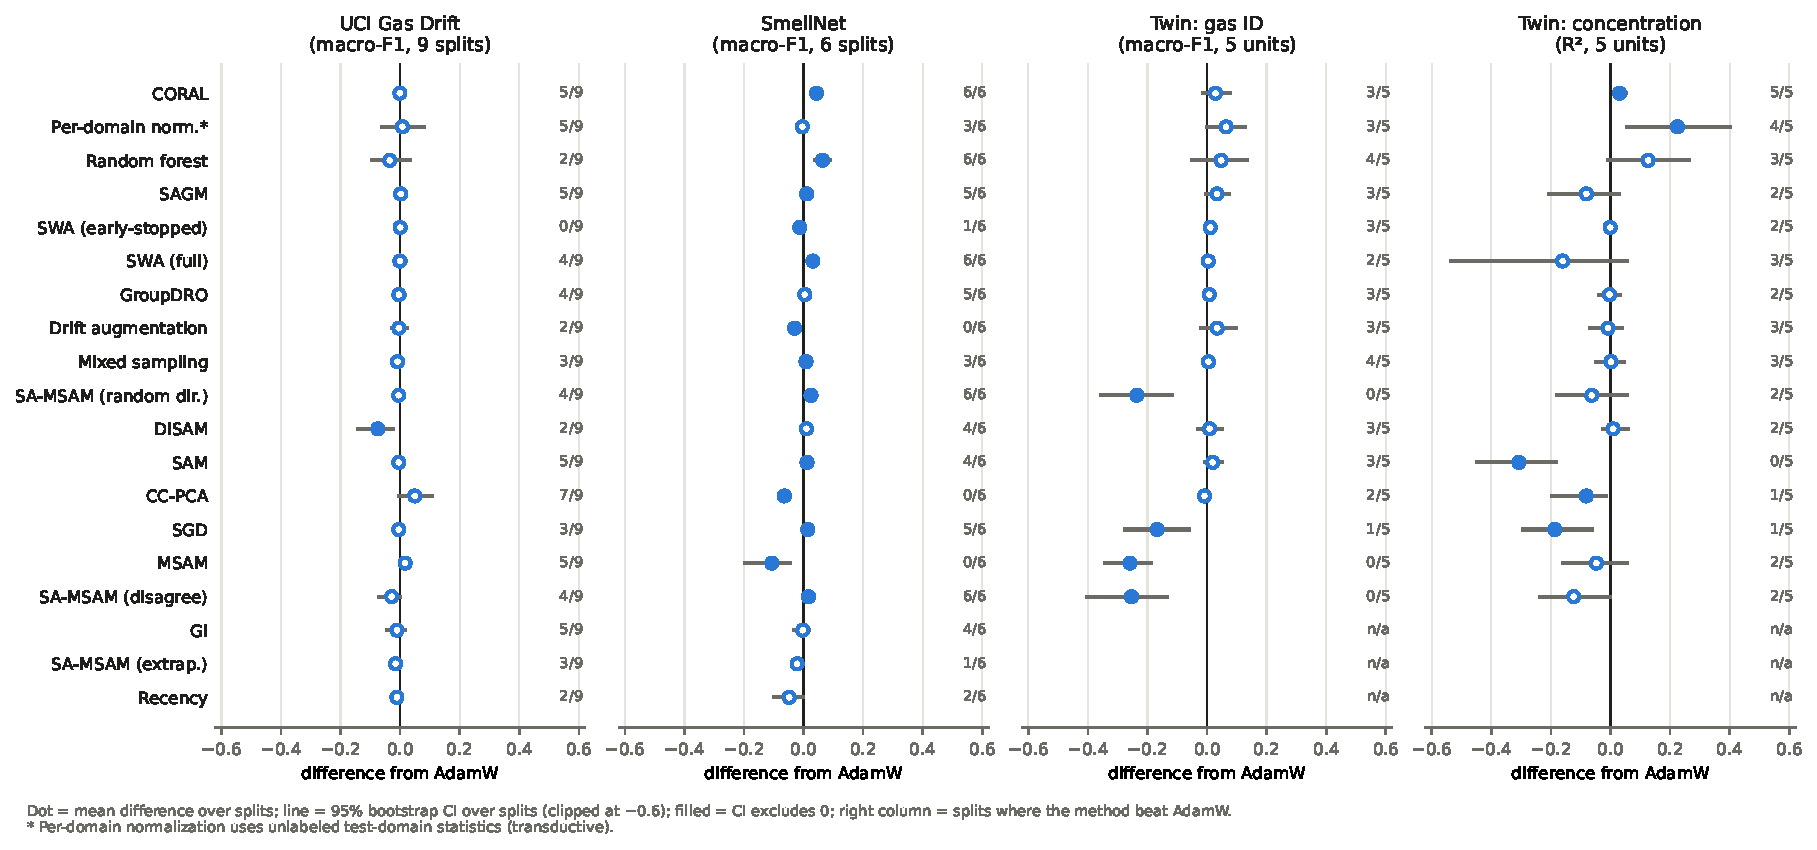
\includegraphics[width=\textwidth]{fig/main_effects.pdf}
\caption{Test score of each method minus AdamW. Dot: mean over held-out splits; line: 95\% bootstrap CI; filled:
CI excludes zero; right column: splits where the method beat AdamW.}
\label{fig:main}
\end{figure*}

\begin{table}[t]
\centering\footnotesize\setlength{\tabcolsep}{3pt}
\begin{tabular}{@{}lcccc@{}}
\toprule
Method & UCI & SmellNet & Twin gas & Twin conc. \\
 & F1 & F1 & F1 & $R^2$ \\
\midrule
AdamW (ref.) & .764 & .810 & .913 & .554 \\
SAM & .759 & .822 & .932 & \textbf{.234} \\
MSAM & .781 & \textbf{.704} & \textbf{.652} & .470 \\
SA-MSAM (disagr.) & .736 & .826 & .659 & .418 \\
SA-MSAM (random) & .759 & .835 & .679 & .457 \\
SAGM & .766 & .820 & .946 & .472 \\
DISAM & \textbf{.689} & .820 & .922 & .563 \\
CORAL & .763 & \textbf{.853} & .942 & .585 \\
Per-domain norm.$^*$ & .772 & .806 & \textbf{.977} & \textbf{.779} \\
CC-PCA & \textbf{.813} & .745 & .904 & .473 \\
SWA (full) & .763 & .841 & .917 & .394 \\
Random forest & .729 & \textbf{.874} & .960 & .680 \\
\bottomrule
\end{tabular}
\caption{Mean test score over held-out splits and seeds. Bold: notable best or worst. $^*$transductive.}
\label{tab:main}
\end{table}

\subsection{No training-time method reliably beats AdamW}
\label{sec:main}
\Cref{fig:main,tab:main} show the main comparison. On \textbf{UCI} (ageing) nothing reliably beats AdamW: CC-PCA has
the best mean (+0.049, 7/9 splits), but its CI includes zero and it fails on SmellNet; DISAM is clearly worse
($-$0.075). On \textbf{SmellNet} (session) the random forest (+0.064) and CORAL (+0.043) win on all 6 splits, while
MSAM collapses ($-$0.106) at its validation-selected learning rate. On \textbf{Twin} (device), gas identification is
near ceiling except that MSAM and SA-MSAM collapse ($\approx-$0.25, 0/5); for concentration, per-device
normalization gives +0.224 $R^2$ (4/5, CI 0.05--0.41) and SAM is worst ($-$0.31). With 5--9 splits no pairwise
difference survives Holm correction (on SmellNet the smallest attainable corrected $p$ is $\approx$0.6), so we rely
on effect sizes, CIs and win counts; Friedman tests reject ``all methods equal'' on every dataset.

\begin{table}[t]
\centering\footnotesize\setlength{\tabcolsep}{4pt}
\begin{tabular}{@{}lcccc@{}}
\toprule
Per epoch & UCI & SmellNet & Twin gas & Twin conc. \\
\midrule
SGD   & 59 / 114 & 45 / 137 & 10 / 29 & 10 / 28 \\
AdamW & 59 / 126 & 45 / 137 & 10 / 28 & 10 / 31 \\
MSAM  & 59 / 176 & 45 / 143 & 10 / 29 & 10 / 36 \\
SAM   & 118 / 358 & 90 / 291 & 20 / 46 & 20 / 52 \\
SAGM  & 118 / 256 & 90 / 279 & 20 / 54 & 20 / 60 \\
DISAM & 114 / 381 & 84 / 360 & 16 / 71 & 16 / 78 \\
\bottomrule
\end{tabular}
\caption{Training cost: forward/backward passes / milliseconds per epoch (median over final runs).}
\label{tab:cost}
\end{table}

\paragraph{Cost.} MSAM delivers its promised saving: it needs the same passes per epoch as SGD and about half the
time of SAM (\cref{tab:cost}). The saving matters little because neither improves robustness.

\subsection{SA-MSAM: a negative result}
\label{sec:samsam}
At the pre-registered validation go/no-go, before any test run, no SA-MSAM variant beat MSAM (UCI $-$0.007 to
$-$0.017; SmellNet $-$0.012 to $-$0.016), and neither drift-direction estimate beat the random-direction control.
Where SA-MSAM looks better than MSAM on test (SmellNet), the difference comes from its lower selected learning rate,
not the direction. A plausible reason is that the drift has no consistent direction: UCI batch 10 reverts towards
batch 1, and SmellNet shift is day-to-day.

\subsection{Selection under drift and the role of flatness}
\label{sec:selection}
We observe four validation$\to$test reversals: recency weighting and MSAM on SmellNet, CC-PCA (best SmellNet
validation score 0.858, second-worst on test) and MSAM on Twin gas (validation 0.996, test collapse). In a selection
study that evaluates all 12 configurations of 8 methods on test (1{,}152 runs; one test split per dataset, so
indicative), validation and test rankings on UCI are slightly opposed (Spearman $-$0.13; $-$0.97 for AdamW), and for
AdamW, DISAM and GroupDRO the validation pick was worse than a random working configuration (\cref{fig:selection}).
Selecting by mean minus standard deviation over seeds reduced the selection regret on SmellNet from 0.040 to 0.013 but
did not help on UCI.

Correlating three sharpness measures (adversarial, top Hessian eigenvalue, random perturbation) with test score
within each split gives weak and inconsistent values: adversarial sharpness $\rho\approx-$0.15 (UCI), $-$0.29
(SmellNet), +0.08 (Twin gas), $-$0.13 (Twin concentration); random-perturbation sharpness $\approx$0. Flatter models
are at most slightly better.

\begin{figure*}[t]
\centering
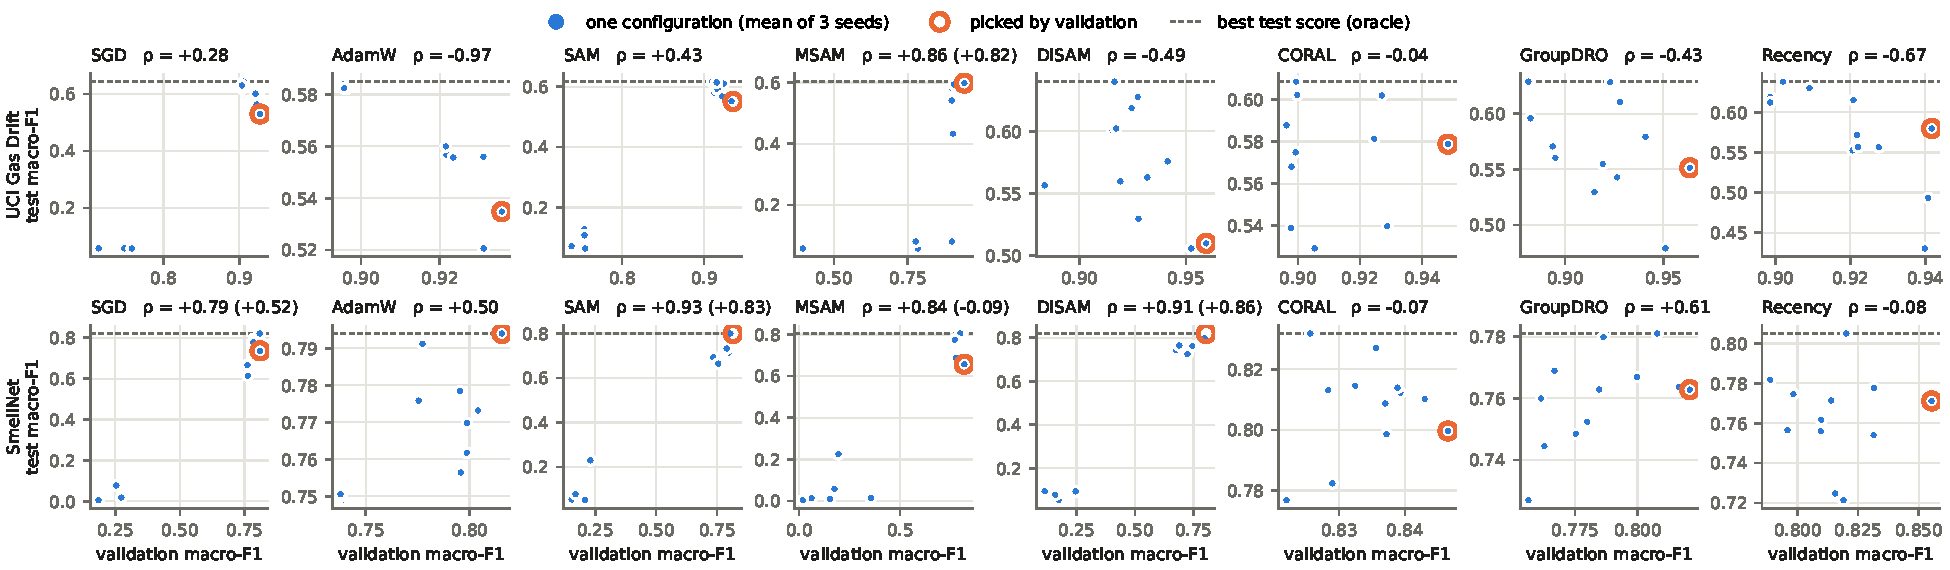
\includegraphics[width=0.9\textwidth]{fig/selection_val_vs_test.pdf}
\caption{Validation (x) vs test (y) score of every configuration (mean of 3 seeds). Ring: validation pick; dashed:
best attainable test score; $\rho$: Spearman correlation.}
\label{fig:selection}
\end{figure*}

\subsection{What kind of drift is it?}
\label{sec:diag}
\begin{table}[t]
\centering\footnotesize\setlength{\tabcolsep}{3.2pt}
\begin{tabular}{@{}lcccc@{}}
\toprule
Dataset & None & Standardize & Oracle & Oracle \\
 & & (label-free) & offset & gain+offset \\
\midrule
Twin gas (F1) & .911 & .965 & .952 & \textbf{.993} \\
Twin conc. ($R^2$) & .576 & .692 & .501 & \textbf{.713} \\
UCI (F1) & .759 & .694 & .785 & .693 \\
SmellNet (F1) & .836 & .802 & .796 & .796 \\
\bottomrule
\end{tabular}
\caption{Shift diagnosis: per-feature input corrections on the test domain. Oracle maps use test labels and are a
diagnostic upper bound only.}
\label{tab:diag}
\end{table}
\Cref{tab:diag} shows that device-to-device shift is almost entirely a per-sensor scale and offset error: an oracle
gain and offset recovers Twin gas identification to 0.993. For ageing, even the oracle calibration does not help, so
the response pattern itself changes. SmellNet is also not repaired by per-feature calibration of the raw input, but
\cref{sec:tta} shows it is largely repaired by adaptation inside the network: its session shift is simple at the
level of learned features rather than raw readings.

\begin{figure*}[t]
\centering
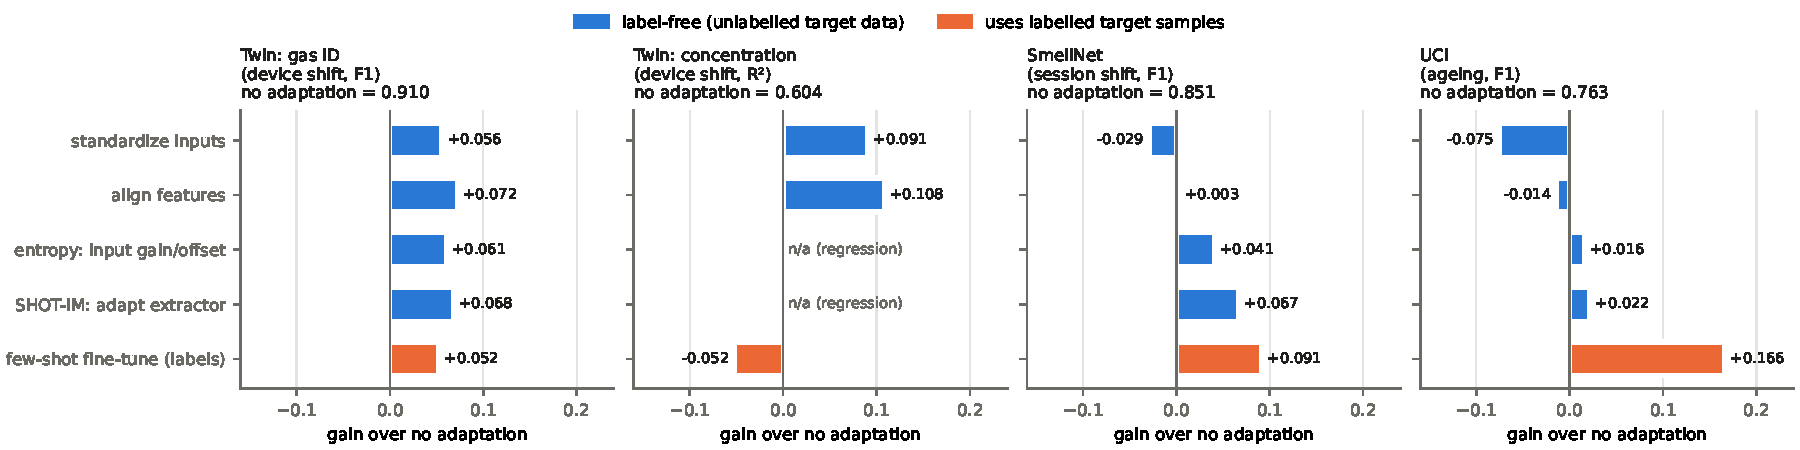
\includegraphics[width=\textwidth]{fig/tta.pdf}
\caption{Gain over the unadapted AdamW model (mean over test splits, 5 seeds). Blue: label-free methods using only
unlabelled target data; orange: few-shot fine-tuning with labelled target samples. Entropy-based methods do not apply
to regression.}
\label{fig:tta}
\end{figure*}

\subsection{Label-free adaptation works for device and session shift, not ageing}
\label{sec:tta}
\begin{table}[t]
\centering\footnotesize\setlength{\tabcolsep}{3pt}
\begin{tabular}{@{}lcccc@{}}
\toprule
Dataset (drift) & None & Best label-free & Few-shot & Wins \\
\midrule
Twin gas (device) & .910 & \textbf{.982} (align) & .962 & 3/5 \\
Twin conc. (device) & .604 & \textbf{.712} (align) & .552 & 4/5 \\
SmellNet (session) & .851 & .918 (SHOT) & \textbf{.943} & 6/6 \\
UCI (ageing) & .763 & .784 (SHOT) & \textbf{.929} & 5/9 \\
\bottomrule
\end{tabular}
\caption{Label-free TTA vs few-shot fine-tuning (5 seeds). Wins: splits where the best label-free method beats no
adaptation (the other two Twin gas splits are at ceiling).}
\label{tab:tta}
\end{table}
On \textbf{device shift} (\cref{fig:tta,tab:tta}), label-free adaptation matches or beats few-shot fine-tuning,
consistent with the calibration-type diagnosis; two labelled recordings per gas are too few to fine-tune the
regression model, whereas aligning feature statistics needs no labels. On \textbf{session shift}, SHOT-IM recovers
$\approx$70\% of the few-shot gain (+0.067 of +0.091) without labels and improves all 6 sessions, while plain input
standardization hurts. On \textbf{ageing}, the best label-free method gains only +0.022 against +0.166 for few-shot
fine-tuning, and every TTA configuration lowers the UCI validation score.

\paragraph{Deciding when to adapt.} A label-free rule---standardize only if this lowers $\mathcal{L}_{\text{IM}}$---chose
correctly on 6/6 SmellNet and 5/5 Twin domains but on only 31\% of UCI domains; a cross-seed agreement rule reached
38\%. Without target labels, a change in the input distribution can come from the sensors or from the gases (a
different class mix or concentrations). Label-free methods assume the class structure is preserved up to a simple
transformation, which holds for calibration offsets between devices but not when ageing changes how each sensor
responds to each gas. The two explanations cannot be separated from unlabelled data alone.

\subsection{Ablations}
\label{sec:ablations}
\begin{table}[t]
\centering\footnotesize\setlength{\tabcolsep}{4pt}
\begin{tabular}{@{}lcc@{}}
\toprule
SmellNet model & AdamW & + CORAL \\
\midrule
1-D CNN, raw windows (main) & .810 & .853 \\
GRU (2$\times$64), raw windows & .820 & .856 \\
MLP, 30 summary features & .842 & .866 \\
Random forest, 30 features & .874 & -- \\
\bottomrule
\end{tabular}
\caption{Architecture vs features on SmellNet (6 held-out sessions $\times$ 5 seeds).}
\label{tab:arch}
\end{table}
\paragraph{Architecture vs features.} Replacing the CNN by a GRU changes the score by +0.010 (4/6 sessions), and by
+0.003 with CORAL (\cref{tab:arch}). CORAL adds $\approx$+0.04 to either network, and per-channel summary features
(mean, standard deviation, min, max, slope) beat both raw-signal networks, so our conclusions are not an artifact of
the CNN.

\paragraph{TTA sensitivity and seeds.} On SmellNet validation, SHOT-IM gains +0.09 to +0.11 for learning rates
$10^{-4}$--$10^{-3}$ and 50--200 steps and fails only at $10^{-2}$ ($-$0.07); on UCI every TTA configuration lowers
the validation score ($-$0.01 to $-$0.08). Three and five seeds give the same TTA numbers within 0.01 (except Twin
concentration feature alignment, 0.736 vs 0.712).

\paragraph{Few-shot budget and SWA.} Gains grow with $k$, and fine-tuning all layers is the most reliable
recalibration (\cref{fig:fewshot}); affine recalibration helps only on Twin and hurts on SmellNet (0/18 runs
improve). Early stopping ended training before SWA began averaging, so early-stopped SWA equals AdamW; full-length
SWA helps on SmellNet (+0.031, 6/6).

\begin{figure*}[t]
\centering
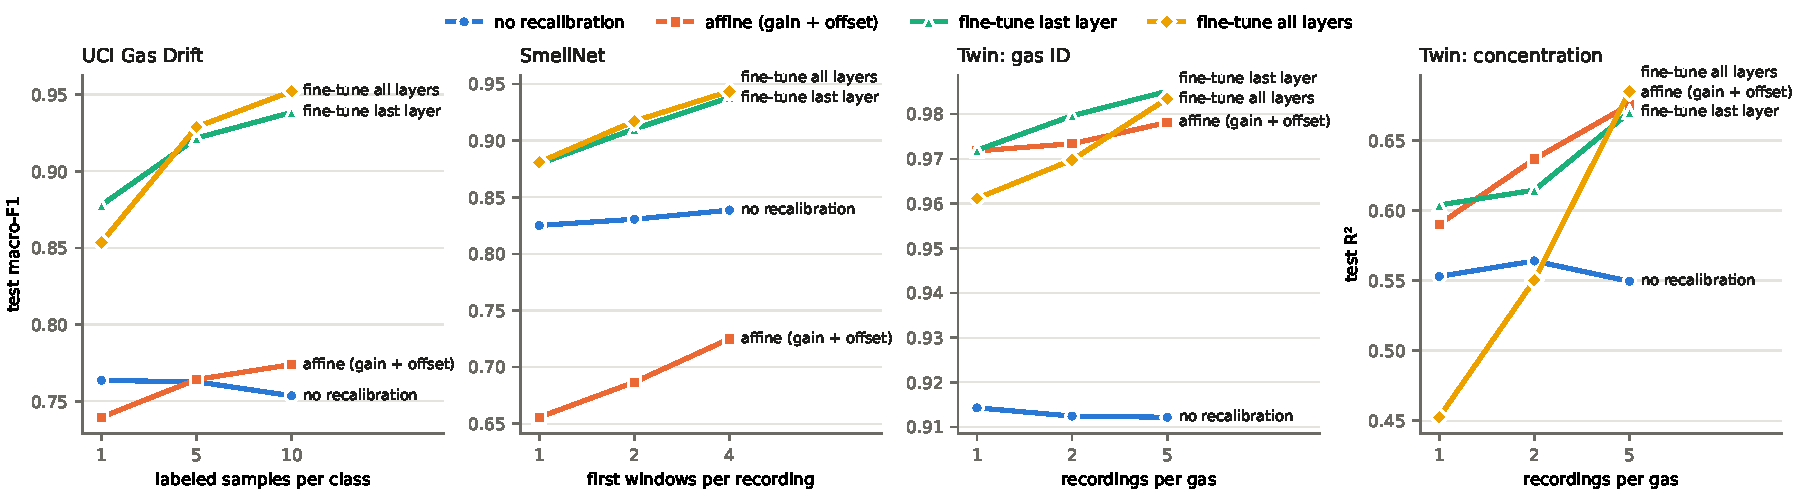
\includegraphics[width=\textwidth]{fig/fewshot.pdf}
\caption{Few-shot recalibration of the frozen AdamW model with $k$ labelled samples from the new batch, session or
device (each method tuned on validation).}
\label{fig:fewshot}
\end{figure*}

% ====================================================================== 7 discussion
\section{Discussion and Limitations}
\label{sec:discussion}
Against the hypotheses of the project brief: MSAM matching SAM (H1) is mixed---MSAM $\geq$ SAM on UCI, but it
collapses on SmellNet and Twin gas; MSAM being cheaper than SAM (H2) is supported; rankings differing between random
and temporal splits (H3) is strongly supported; and benefits varying by batch (H4) is supported. More broadly, across
$\approx$7{,}200 runs the method family mattered far less than the drift type. Training-time robustness gives at most
small, dataset-specific gains. When the shift is calibration-type, cheap label-free adaptation recovers most of the
loss; for ageing, labelled target samples are needed. The oracle-calibration diagnosis, run on a small labelled set
from the new condition, indicates which case applies.

\paragraph{Limitations.} Few held-out domains (5--9 per dataset) limit statistical power, and the selection study
uses one test split per dataset. Some baselines (random forest, full-length SWA) were added after early test results
were seen; this is disclosed and they received the same tuning budget. Per-domain normalization and TTA are
transductive. The UCI release lacks the pre-exposure baseline needed to rule out the confound
of~\cite{dennler2022drift}, and SmellNet's session order is assumed chronological. Only small models were used, and
prior e-nose TTA methods~\cite{liang2024otta,liang2025otta} were not re-implemented.

% ====================================================================== 8 reproducibility
\section{Reproducibility}
\label{sec:repro}
\paragraph{Code and environment.} All code, results and checkpoints are at\\
\mbox{\href{https://github.com/RahulBhikundia/enose-drift-benchmark}{\footnotesize\texttt{github.com/RahulBhikundia/enose-drift-benchmark}}}.\\
Library code (loaders, models, optimizers, the single-run trainer) is in \texttt{src/}; drivers are
grouped by role in subfolders of \texttt{scripts/} (\texttt{data}, \texttt{experiments}, \texttt{analysis},
\texttt{figures}, \texttt{report}, \texttt{orchestration}). The environment is
given as \texttt{environment.yml} (conda) and \texttt{requirements.lock.txt} (exact pip versions: Python 3.12.8,
PyTorch 2.5.1+cu121, scikit-learn 1.5.2). All runs used one NVIDIA GTX 1650 (4\,GB) under Windows 11; they also run
on CPU. \texttt{tests/test\_optim.py} checks our MSAM against the official implementation step by step.

\paragraph{Data.} The three datasets are public and are not stored in the repository (3\,GB).
\texttt{scripts/data/download\_data.py} fetches UCI \#224 and \#361 and SmellNet (Hugging Face, pinned commit
\texttt{45405fe}) and verifies SHA-256 checksums listed in \texttt{data/README.md}.

\paragraph{Artifacts.} Each of the 7{,}194 training runs (about 18 GPU-hours) is stored as a JSON file holding its
arguments, seed, library versions, GPU, timing, learning curve, per-domain metrics and test predictions. Every table
and figure is regenerated from these files by \texttt{scripts/analysis} and \texttt{scripts/figures}; frozen
hyperparameter selections are in \texttt{results/tuning/selected\_*.json}, and dated decisions and pre-registrations
in \texttt{notes/decisions.md}. The README lists the commands in order.

\paragraph{Checkpoints.} All models are small (35k--67k parameters), so the repository ships weights instead of a
link: the seed-0 model of SGD, AdamW, SAM and MSAM for every held-out split (97 files; 3 runs diverged in the original study), each with its arguments, in
\texttt{checkpoints/}. Other models are fully specified by their JSON files and re-train in seconds to minutes.
To produce them we re-trained the 97 non-diverged runs from their stored arguments and compared test scores with
the reported ones (\cref{tab:rerun}). All 73 MLP runs (UCI, Twin) reproduce the reported score exactly. The SmellNet
CNN does not, because seeds are fixed but cuDNN convolution kernels are not forced to be deterministic: the median
difference is 0.018, below the seed-to-seed spread, but one MSAM run (loso6) collapsed on re-training (0.733
$\rightarrow$ 0.187), the same instability reported in \cref{sec:main}. This is why every claim in this report is
made over seeds and splits, never from a single run.

\begin{table}[t]
\centering\small
\begin{tabular}{@{}lrrrrr@{}}
\toprule
 & & \multicolumn{2}{c}{$|$re-run $-$ reported$|$} & seed SD & MB \\
\cmidrule(lr){3-4}
Dataset & ckpts & median & max & median & \\
\midrule
UCI (ageing) & 36 & 0.000 & 0.000 & 0.037 & 9.7 \\
SmellNet & 24 & 0.018 & 0.546 & 0.031 & 3.4 \\
Twin gas & 20 & 0.000 & 0.000 & 0.085 & 4.1 \\
Twin conc. & 17 & 0.000 & 0.000 & 0.208 & 3.5 \\
\bottomrule
\end{tabular}

\caption{Re-training check of the 97 shipped checkpoints: absolute difference between the re-trained and the
reported test score (macro-F1; $R^2$ for Twin concentration), next to the median standard deviation over seeds of
the same runs. Generated by \texttt{scripts/report/make\_repro\_tex.py} from \texttt{checkpoints/manifest.csv}.}
\label{tab:rerun}
\end{table}

\paragraph{Commit history.} \cref{tab:commits} lists the repository's commits. The project was developed locally
with a dated log (\texttt{notes/progress\_log.md}, 11--26 Nov 2026) and placed under version control for submission,
so the timestamps record when each part was committed, not when it was written. The commit that adds this table
follows the ones listed; \texttt{git log} in the repository is authoritative.

\begin{table}[t]
\centering\footnotesize
\begin{tabular}{@{}l l l p{0.40\linewidth}@{}}
\toprule
Commit & Time (IST) & Author & Content \\
\midrule
\texttt{9a39c10} & 26 Nov 20:44 & Rahul & Project setup: environment files, dataset provenance and download script \\
\texttt{7b4a034} & 26 Nov 21:01 & Rahul & UCI drift and SmellNet loaders with leakage audits \\
\texttt{9dc5ea1} & 26 Nov 21:02 & Rahul & Models, single-run trainer, SAM / MSAM / SA-MSAM and MSAM equivalence test \\
\texttt{a72c0ee} & 26 Nov 21:03 & Rahul & Equal-budget tuning grid and frozen validation-only selection for the optimizers \\
\texttt{d3bdd95} & 26 Nov 21:03 & Rahul & Frozen test runs and statistics for the optimizers (UCI, SmellNet) \\
\texttt{c628ed3} & 26 Nov 21:20 & Gourav & Domain-generalization baselines: SAGM, DISAM, CORAL, GroupDRO, per-domain normalization \\
\texttt{fb3e65f} & 26 Nov 21:21 & Gourav & CC-PCA, drift augmentation and SWA (with full-length SWA re-selection) \\
\texttt{bb38d2c} & 26 Nov 21:21 & Gourav & Test runs for the DG baselines and the random-forest baseline \\
\texttt{9527a9c} & 26 Nov 21:22 & Gourav & Twin gas sensor arrays: loader, device-shift audit, tuning and 10-seed test runs \\
\texttt{e4ef302} & 26 Nov 21:23 & Gourav & Model-selection study: validation vs test rankings under drift \\
\texttt{4ff886b} & 26 Nov 21:40 & Jharendra & Shift diagnosis by oracle per-feature gain/offset calibration \\
\texttt{91a240b} & 26 Nov 21:41 & Jharendra & Few-shot recalibration with k labelled target samples \\
\texttt{5497911} & 26 Nov 21:41 & Jharendra & Label-free test-time adaptation: standardize, feature alignment, IM affine, SHOT-IM \\
\texttt{66147cb} & 26 Nov 21:42 & Jharendra & Ablations: feature MLP and GRU on SmellNet, TTA hyperparameter sensitivity \\
\texttt{ca4c2c4} & 26 Nov 21:42 & Jharendra & Seed-0 checkpoints for SGD/AdamW/SAM/MSAM and re-training check \\
\bottomrule
\end{tabular}

\caption{Commits in the project repository (short hash, date and time, author, content). Generated from \texttt{git log}.}
\label{tab:commits}
\end{table}

\paragraph{Declaration.} We declare that every number in this report was produced by the code in the repository
above, on the public data described in \cref{sec:data}, under the protocol of \cref{sec:protocol}; that no test
result was used to choose a method, hyperparameter, epoch count or seed; and that analyses added after test results
were seen are marked as such (\cref{sec:discussion}). The per-run JSON files, frozen selections and checkpoints are
sufficient to regenerate every table and figure without retraining.

% ====================================================================== 9 conclusion
\section{Conclusion}
\label{sec:conclusion}
Under a leakage-free, validation-only protocol, sharpness-aware optimizers---including the cheap MSAM and our
drift-aware variant---do not make gas-sensor classifiers robust to real drift, and validation scores are an
unreliable guide under drift. The more useful question is what kind of drift is present: device and session shifts
can be absorbed by label-free test-time adaptation, while ageing needs a few labelled samples from the new period. A
simple oracle-calibration diagnosis tells the cases apart.


{
    \small
    \bibliographystyle{ieeenat_fullname}
    \bibliography{main}
}

\end{document}
